\title{Decidable Subtyping\\ of Existential Types\\for the Julia Language}
% \subtitle{Restricting Existential Types Inside Invariant Constructors\\ 
% to Use-Site Variance}

\author{Julia Belyakova}

\date{\normalsize%
\vfill
\vspace{6cm}
Submitted in partial fulfillment of the requirements\\
for the degree of Doctor of Philosophy\\
\vspace{1em}
Khoury College of Computer Sciences\\
Northeastern University\\
Boston, Massachusetts, USA\\
\vspace{1em}
August 2023
}

\maketitle

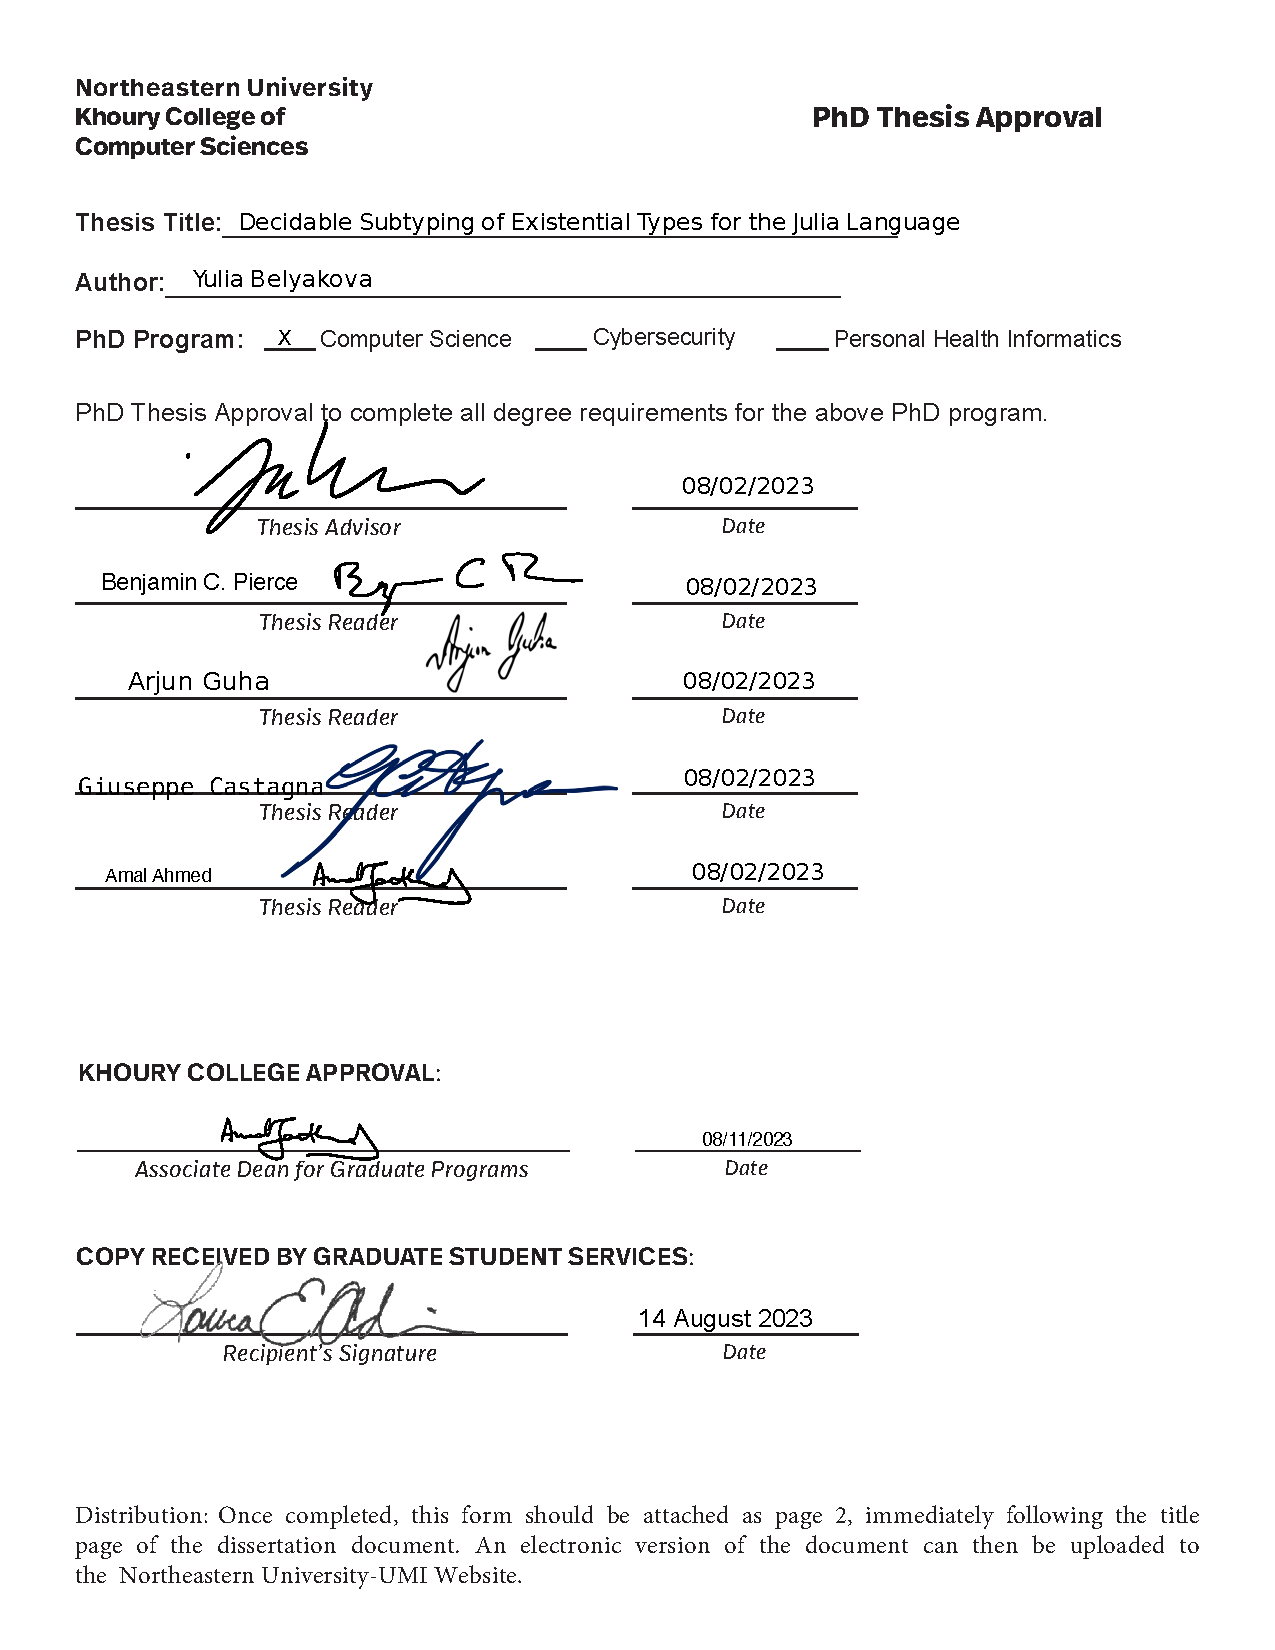
\includepdf[noautoscale]{approval.pdf}

\begin{abstract}

Julia is a dynamic, high-performance programming language
for scientific computing.
To encourage a high level of code reuse and extensibility, Julia is
designed around symmetric multiple dynamic dispatch, which allows functions
to have multiple implementations tailored to different argument types.
To resolve multiple dispatch, Julia relies on a subtype relation over a complex
language of run-time types and type annotations, 
which include set-theoretic unions, distributive tuples, parametric invariant 
types, and impredicative existential types.
Notably, subtyping in Julia is undecidable, which
manifests with a run-time stack-overflow error when program execution encounters
a subtyping query that causes the subtype checker to loop.

In this dissertation, I propose a decidable subtype relation for a restricted
language of Julia types where existential types inside invariant constructors
are limited to ones expressible with use-site variance.
To estimate the migration effort that would be required for switching to the 
restricted type language, I analyze type annotations in the corpus of 9K
registered Julia packages.
Out of 2M statically identifiable type annotations in the corpus,
99.99\% satisfy the restriction, making it a viable candidate for
evolving Julia towards decidable subtyping.

\end{abstract}
